El dispostivo experimental diseñado para la realización del estudio de caracterización de estas fibras se muestra de forma esquemática en la figura \ref{esquemasetup}.

\begin{figure}[H]
\centering
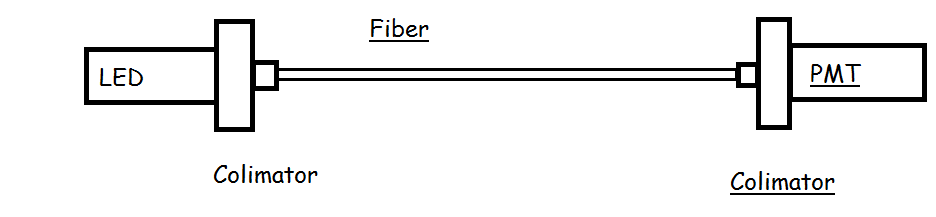
\includegraphics[scale=0.45]{Figuras/Set_up.png}
\caption{Esquema del dispositivo experimental utilizado en el estudio\label{esquemasetup}}
\end{figure}

El dispositivo esperimental esta formado por 5 piezas distintas:
\begin{itemize}
\item {} En primer lugar podemos observar la existencia de un diodo LED, el cual actuará como fuente de fotones. Con ayuda de un espectrómetro existente en los laboratorios del ICMOL se ha realizado un espectro de los fotones emitidos por el diodo LED el cual puede observarse en la figura \ref{espectroled}

\begin{figure}[H]
\centering
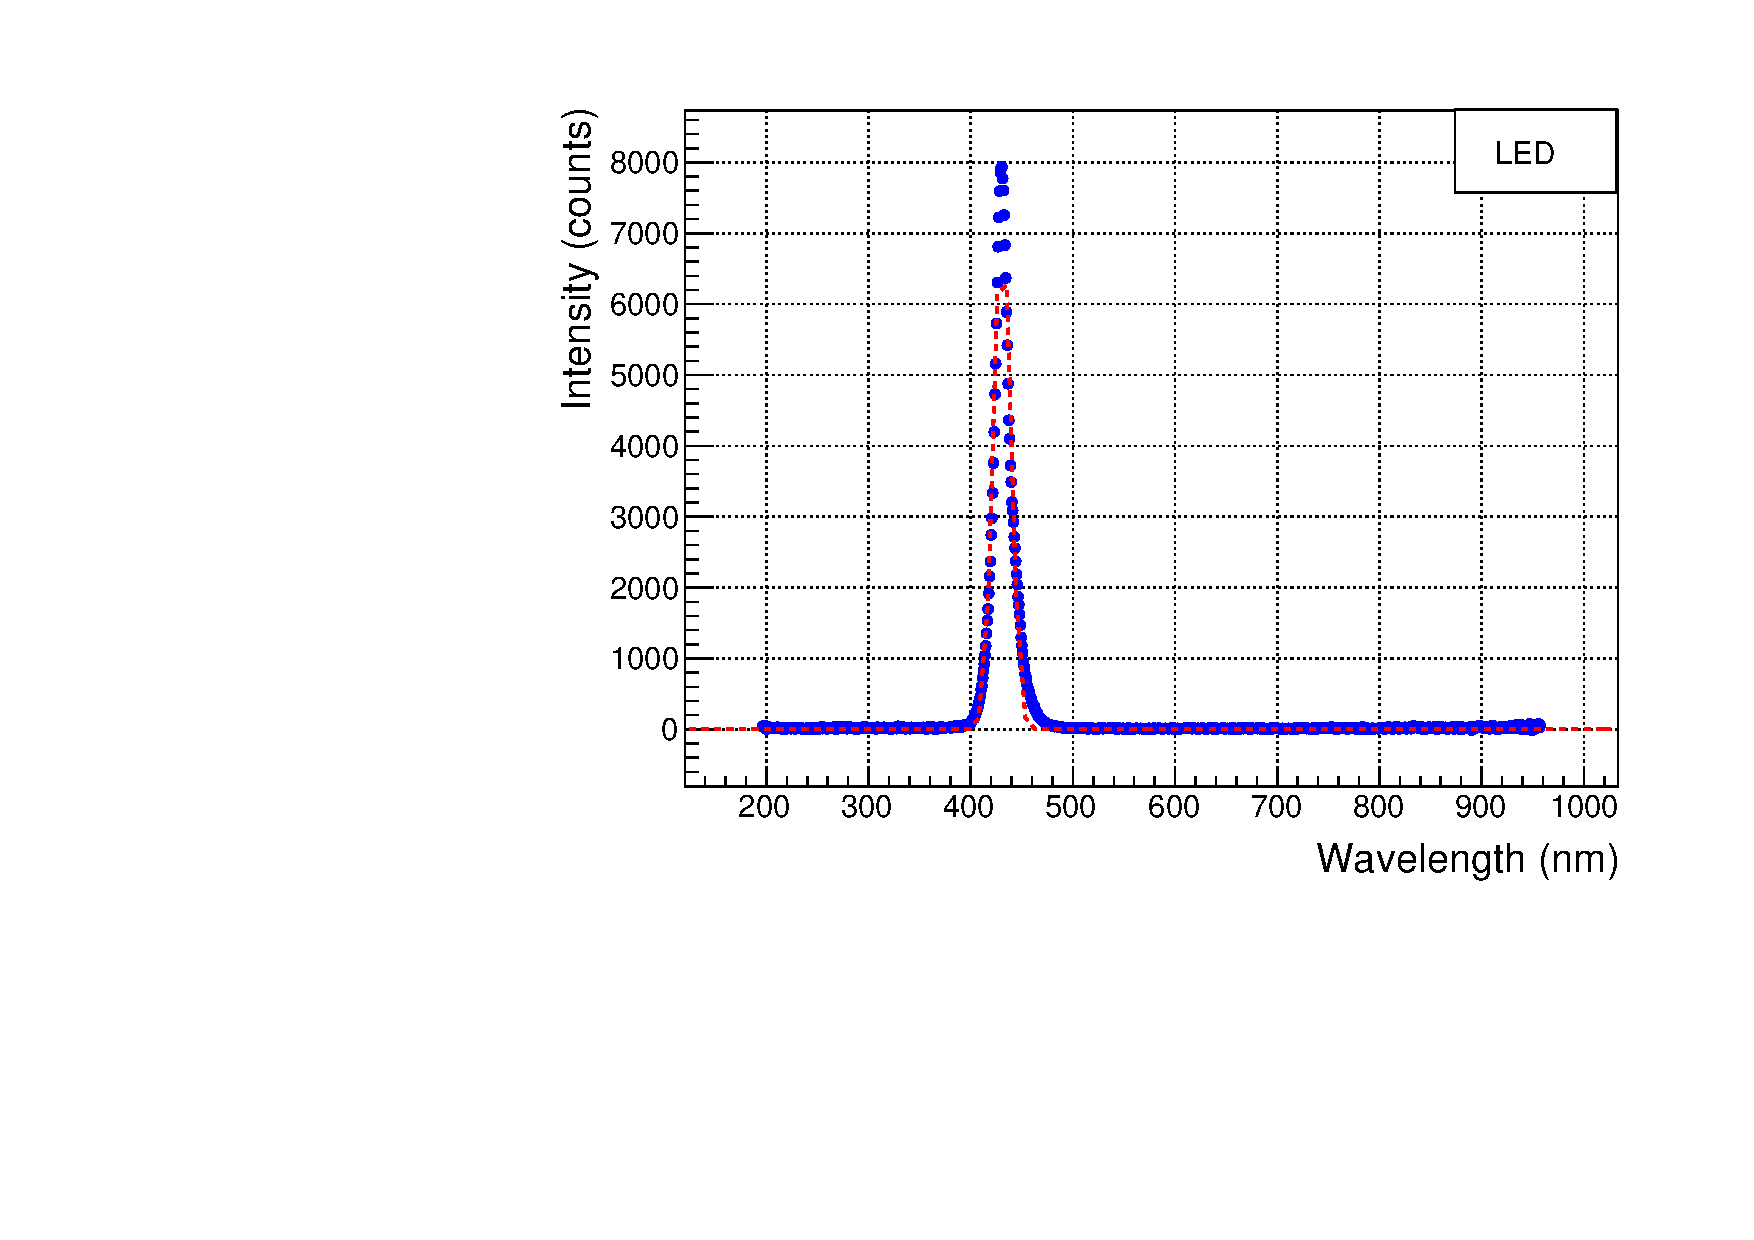
\includegraphics[scale=0.7]{Figuras/Plot_LED.pdf}
\caption{Espectro del diodo LED empleado en el dispositivo experimental\label{espectroled}}
\end{figure}

En este podemos comprobar que la emisión del diodo led posee un pico bastante estrecho el cual, con ayuda de un ajuste a una gaussiana, observamos que se encuentra en $\lambda=430,8 \pm 0.1$ con una anchura de $\sigma_{\lambda}=8.3\pm0.1$. La razón de ello es que queremos caracterizar las fibras en este intervalo del espectro debido a que este es el intervalo de interes desde el punto de vista del proyecto Tritium ya que nos encontramos muy cerca del pico de emisión que presentan la fibras empleadas en el estudio (BCF-12), el cual se encuentra entorno a $\lambda=435~\nano\meter$.

\item{} Un tubo fotomultiplicador (PMT) con el que leeremos el número de fotones que recibamos del sistema. El PMT utilizado es Hamamatsu R8520-ZB2771, cuya eficiencia a la longitud de onda de trabajo es de $\epsilon=29.76\%$. Este se encuentra alimentado a $250~\volt$ y posee un cortocircuito en el sistema de dinodos que le permite acturar con ganancia 1.

\item{} La fibra sometida a estudio se situará entre ambos dispositivos anteriormente mencionados, el diodo LED y el PMT. El objetivo de este es que la señal que midamos provenga de los fotones emitidos por el diodo LED tras haber cruzado la fibra centelleadora. Dado que con el estudio anterior sober el diodo LED tenemos bien caracterizada su señal, con este sistema podremos quantificar la eficiencia de colección que presenta cada tipo de fibra ademas de sus posibles incertidumbres procedentes de diversas fuentes.

Hay que tener en cuenta que la longitud activa de la fibra en la que se estudiará la caracterización de estas es lijeramente menor que la longitud total. El motivo de ello es que una pequeña parte de estas (aproximadamente $4~\mm$ a cada lado) son empleados para cruzar el conector y realizar un contacto opticamente aceptable con el PMT con ayuda de grasa óptica. Estas pequeñas longitudes se encuentran recubiertas por finas capas de teflón (politetrafluoroetileno) el cual posee un coeficiente de reflexión de prácticamente el $100\%$ con fotones en el rango del visible, com es nuestro caso. Esto se realiza para evitar añadir la incertidumbre del tramo del interior del conector ya que estos son metálicos y solo nos interesa realizar la caracterización en un medio aéreo. En trabajo, siempre que hablemos de longitud, nos estaremos refiriendo a la longitud activa de la fibra. En caso contrario se especificará.

\item{}Seguidamente queremos asegurar que los fotones medidos por el tubo fotomultiplicador procedan únicamente del diodo LED tras haber cruzado la fibra. Para ello introducimos un primer colimador justo antes del PMT, de esta manera seguramos que los fotones que medimos proceden del interior de la fibra y un segundo colimador justo despues de la LED. Con esta configuración podemos asegurar que la procedencia de estos fotones es la adecuada. Ambos colimadores han sido específicamente construidos en los talleres del IFIC para este estudio por lo que posee una colimación perfecta.

\item{} Finalmente se emplearan unos conectores comerciales obtenidos de la empresa Saint-Gobain para sujetar de forma segura estas fibras, tanto en el dispositivo experimental como en las diversas labores que así lo requieran como por ejemplo el pulido. Estos conectores pueden verse en la figura \ref{conector}.

\begin{figure}[H]
\centering
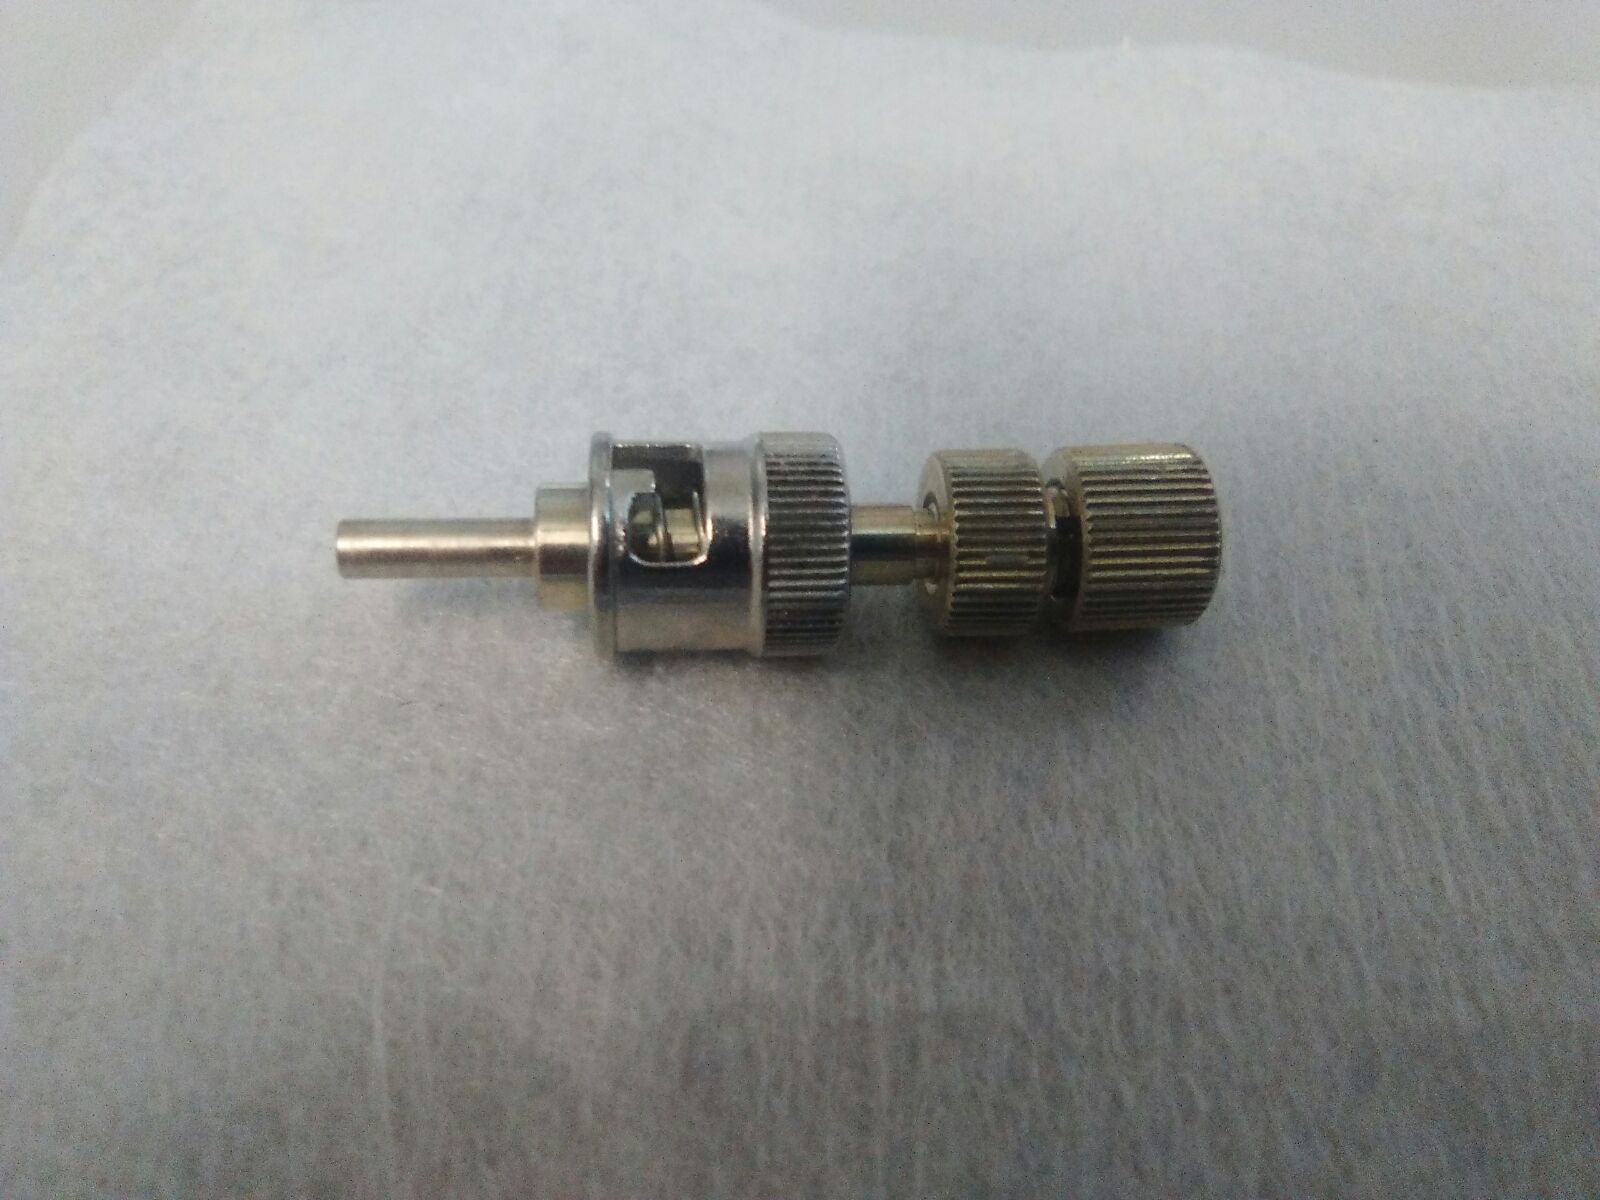
\includegraphics[scale=0.1]{Figuras/conector.jpeg}
\caption{Conector comercial empleado para la sujeción de la fibra\label{conector}}
\end{figure}

Hay que tener en cuenta que, dado que estos conectores son metálicos, se utilizaron finas capas de teflón entre la fibra y el conector para evitar daños en la fibra.




\end{itemize}
